
\section{Modelo ARIMA Auto}
Finalmente, se realiza un modelo ARIMA utilizando los valores obtenidos por el siguiente código. Este encontrará los valores más óptimos para la creación del modelo.

\begin{lstlisting}
	modelo = auto_arima(
	y                 = train,
	start_p           = 0,
	start_q           = 0,
	max_p             = 3,
	max_q             = 3,
	seasonal          = True,
	test              = 'adf',
	m                 = 7, # periodicidad de la estacionalidad
	d                 = None, # El algoritmo determina 'd'
	D                 = None, # El algoritmo determina 'D'
	trace             = True,
	error_action      = 'ignore',
	suppress_warnings = True,
	stepwise          = True
	)
\end{lstlisting}

Se obtiene el siguiente resultado:
\begin{figure}[!h]
	\centering
	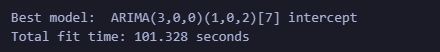
\includegraphics[width=0.7\linewidth]{arima_auto_optimo}
	\caption{Valores Óptimos Arima Auto}
	\label{fig:arimaautooptimo}
\end{figure}
La expresión algebraica para representar SARIMAX(1,1,1)(1,1,1,7) sería:
\begin{equation}[h]
	(1 - \phi_1L)\cdot(1 - \Phi_1L^7)\cdot(1 - L)Y_t = (1 - \theta_1L)\cdot(1 - \Theta_1L^7)\cdot \epsilon_t
\end{equation}

Estos se insertan en el código y obtenemos la siguiente figura. Como Se puede apreciar tanto el ARIMA que se ha deducido como el ARIMA auto se asemejan mucho a los valores reales de TEST.

\begin{figure}[!h]
	\centering
	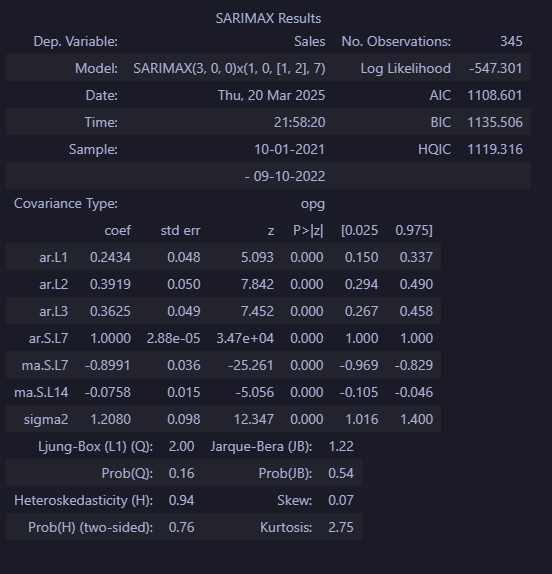
\includegraphics[width=0.5\linewidth]{sarimax_auto_resultados}
	\caption{Arima Auto}
	\label{fig:sarimaxautoresultados}
\end{figure}

El código anterior permite calcular el intervalo de confianza y muestra las predicciones. Como podemos ver las predicciones se encuentrar del intervalor de confianza para la mayoria de las predicciones. sto significa que, con un 95\% de confianza, las ventas reales para ese día caerán dentro de este rango.

\begin{figure}[!h]
	\centering
	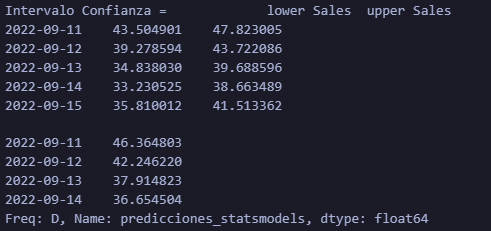
\includegraphics[width=0.5\linewidth]{confianza_sarimax_auto}
	\caption{Intervalo de Confianza y Predicción Arima Auto}
	\label{fig:confianzasarimaxauto}
\end{figure}

La figura muestra las predicciones del modelo SARIMAX auto y manual junto con las muestras de test reales. Ambos modelos se ajustan muy bien al verdadero.

\begin{figure}[!h]
	\centering
	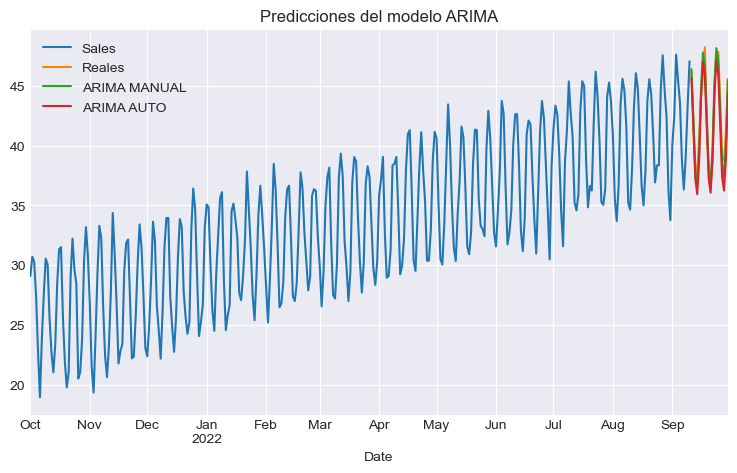
\includegraphics[width=0.7\linewidth]{auto_arima}
	\caption{Gráfico Arima Auto}
	\label{fig:autoarima}
\end{figure}


\subsection{Validación}
Se observa que la los valores obtenidos como errores son  bajos. Tomando 45 como el promedio de $Sales$ para la predicción, el MSE y MAE dde 1.871 y1.141 respectivamente indican un error de alrededor del 4.16\% y 2.53\%, mientras que el RMSE de 1.37 indica un error de aproximadamente 3.04\%, estos son mucho más elevados que los dos modelos anteriores.
\begin{figure}[h]
	\centering
	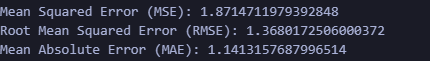
\includegraphics[width=0.7\linewidth]{errores_auto_arima}
	\caption{Errores de Arima Auto}
	\label{fig:erroresautoarima}
\end{figure}

\clearpage

\section{Conclusion}

De acuerdo con las métricas de error (MAE, MSE, RMSE) y la figura 22, el modelo \textbf{ARIMA manual} es el más preciso, con los valores más bajos en todas las métricas disponibles. El modelo Holt-Winters también muestra buen rendimiento en MAE, aunque carece de métricas completas para una comparación más exhaustiva. Por otro lado, el modelo ARIMA Auto presenta los peores resultados, especialmente en MAE, MSE y RMSE, lo que sugiere un rendimiento inferior. En resumen, \textbf{ARIMA manual} es el modelo más adecuado para las predicciones de esta serie temporal.

\begin{figure}[!h]
	\centering
	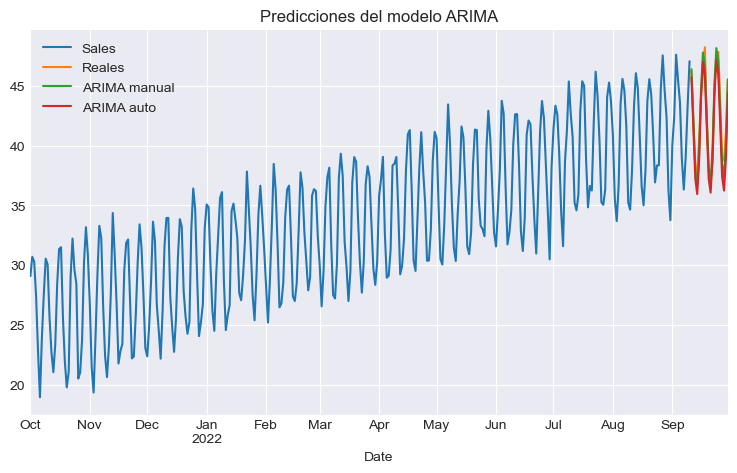
\includegraphics[width=0.8\linewidth]{eleccionModleo.png}
	\caption{Gráfico de elección del modelo}
	\label{fig:eleccionmodleo}
\end{figure}

\begin{table}[h]
	\centering
	\begin{tabular}{| c | c | c | c |}
		\hline
		\textbf{MODELO} & \textbf{MAE} & \textbf{MSE} & \textbf{RMSE} \\ \hline
		Holt-Winters & 0.704 & - & - \\ \hline
		Holt-Winters-Trans & 1.228 & - & - \\ \hline
		ARIMA Manual & 0.690 & 0.694 & 0.830 \\ \hline
		ARIMA Auto & 1.871 & 1.141 & 1.368 \\ \hline
	\end{tabular}
	\caption{Comparación de modelos}
	\label{tab:comparacion_modelos}
\end{table}

\clearpage
\section{Bibliografia}
{https://www.kaggle.com/datasets/sudipmanchare/simulated-sales-data-with-timeseries-features

